%------------------------------------------------------------------------------
% IPOL LaTeX style guide and Example
% by rafael grompone von gioi, nicolas limare, jose-luis lisani and others
%------------------------------------------------------------------------------

% IPOL class is based on the standard LaTeX article class is used
% essentially in the same way. The layout must not be changed. Special
% IPOL commands are used to set the title, authors and abstract.

\documentclass{ipol}

% Do not use math notations and greek letters in the title.
\ipolSetTitle{IPOL Style Guide and Example}

% Author names must be separated with commas (,), not "and" or "&".
\ipolSetAuthors{First Author \ipolAuthorMark{1},
                Second Author\ipolAuthorMark{2}}

% Affiliations must contain the department, institution and country.
% Use a professional email address (no gmail, yahoo, etc).
% Do not add postal address.
\ipolSetAffiliations{%
\ipolAuthorMark{1} Department, Institution, Country
                   (\texttt{user@server.net})\\
\ipolAuthorMark{2} Department, Institution, Country
                   (\texttt{username@mailserver.edu})}

%------------------------------------------------------------------------------

% The link hereafter points to IPOL documentation for convenience
% in this document but must be replaced in your manuscript.
% The preprint link will not be known before the first preprint page
% is created. For early preprint versions, just don't use this command
% and the link will be set to the IPOL journal DOI address.
\ipolPreprintLink{http://www.ipol.im/}

%------------------------------------------------------------------------------

% Add packages and definitions here.
% Keep the package list as small as possible and include the package
% sources (packagename.sty) with your article source.
% These packages are loaded by the IPOL class or considered standard,
% and need not be provided with their source if they are used:
%   color, hyperref, graphicx, rotating
%   amsmath, amssymb, amsthm
% For algorithms, please use the algorithm2e package instead of
% algorithmx for simplicity and a uniform style.

\usepackage[vlined,ruled]{algorithm2e}
% define input and output keywords
\SetKwInOut{Input}{input}
\SetKwInOut{Output}{output}
% define comment style
\SetKwComment{Comment}{}{}
\newcommand{\mycmtsty}[1]{\em \small #1}
\SetCommentSty{mycmtsty}

% Use \newtheorem{} for remarks and definitions.
\usepackage{amsthm}
\newtheorem{definition}{Definition}
\newtheorem*{remark}{Remark}

%------------------------------------------------------------------------------

\usepackage{fancyvrb}
\VerbatimFootnotes % allows verbatim text in footnotes

\begin{document}

% IPOL encourages authors to do joint submissions to IPOL and
% SIIMS (SIAM Journal of Imaging Science). Upon acceptance, cross
% references are placed between both articles. The environment
% ipolSIIMS is used to set the standard header, before the
% abstract. Uncoment these lines if you prepare an IPOL+SIIMS article:

%\begin{ipolSIIMS}
%This IPOL article is related to a companion publication in the SIAM
%Journal on Imaging Sciences:\\
%Author Names, ``Article Title.''
%\textsl{SIAM Journal on Imaging Sciences}, vol.~X, no.~X,
%pp.~N--M, YYYY. \url{https://doi.org//10.1137/XXXXXXXXX}
%\end{ipolSIIMS}

%------------------------------------------------------------------------------
% The abstract of an IPOL article must be informative and summarize all
% important parts of the article. 

\begin{ipolAbstract}
The abstract should contain about 100 to 150 words, and should be
identical to the abstract text submitted electronically. An abstract
must be able to stand alone, independent of the paper.  Written in
plain text, it cannot contain citations to the paper’s references or
equations or footnotes and should not, if possible, include special
characters like math notations or greek letters, or hyperlinks. The
abstract must be a single paragraph; multiple parts can be split with
a single line break.
\end{ipolAbstract}

%------------------------------------------------------------------------------
% Use the source code info to briefly explain what can be found as
% software code in the IPOL article.
% Do not use the phrasing "...the IPOL web part of this article."

\begin{ipolCode}
The source code section briefly explains what the source code
published with the article contains, all in a single paragraph. For
example: The reviewed source code and documentation for this algorithm
are available from \href{\ipolLink}{the web page of this
  article}. Compilation and usage instruction are included in the
\verb|README.txt| file of the archive.
\end{ipolCode}


%------------------------------------------------------------------------------
% Use the supplementary files info to add explanations about other
% files published with the article.

\begin{ipolSupp}
The supplementary files section provides explanations about other
files published with the article, all in a single paragraph. Mention
clearly if they are reviewed or not. For example: A reference dataset,
to be used for further comparisons, is provided with the article and
peer-reviewed. A Matlab interface (not reviewed) is also available for
convenience.
\end{ipolSupp}

%------------------------------------------------------------------------------
% All papers need key words. Key words are lowercase except for proper
% names and acronyms, and separated with commas. Only use plain text.

\ipolKeywords{first, second, third, fourth}

%------------------------------------------------------------------------------
% Article content starts here.

\section{Introduction}

The submission process is detailed in the IPOL
\href{https://tools.ipol.im/wiki/ref/author\_manual/}{Author Manual}. 
Prepare IPOL articles with the \LaTeX\ class available from
\url{\ipolLink}. Just copy \verb|ipol.cls| and the logo
files (\verb|ipol_logo.pdf| and \verb|ipol_logo.eps|, plus
\verb|siims_logo.eps| or \verb|siims_logo.jpg| for IPOL+SIIMS
articles) in the directory containing your manuscript source. Then use
this class like the standard ``article'' class of \LaTeX, with special
commands explained hereafter. You can start by editing the source of
this style guide. Submit your manuscript for review as a PDF file
following this style guide. For review, only the PDF file is needed.

After review and during the editing process, you must provide the
complete source as a single archive file (\verb|zip| or
\verb|tar/gzip|), including the \LaTeX\ source (\verb|.tex|), BibTeX
references (\verb|.bib|), \LaTeX\ class (\verb|.cls|) and style
(\verb|.sty|) and all the graphics files (\verb|.png|, \verb|.jpg|,
and \verb|.pdf|). Remove unused files (including backup and temporary
versions and dotfiles). Please rename your \LaTeX\ source to
\verb|article.tex|. Use plain ASCII text, and \TeX\ commands for
accents (\verb|J\'er\^ome|). This source will be used to produce the
final published PDF version, and must compile with pdf\LaTeX.

\subsection{Title and Authors}

Commands \verb|\ipolSetTitle|, \verb|\ipolSetAuthors| and
\verb|\ipolSetAffiliations|, from the IPOL class, set information
needed to generate the article header and metadata. Use these commands
in the preamble of the \LaTeX\ file, between
\verb|\documentclass{ipol}| and \verb|\begin{document}|.

Do not use special characters (math symbols, superscripts, greek
letters \ldots) in the title if possible. Use headline-style
capitalization for the article title: capitalize the first letter of
the first and last words of the title and subtitle and all other
words, except for articles, coordinating, the words ``to'' and ``as'',
prepositions (unless they are emphasized or used as adverbs,
adjectives, or conjunctions).

Multiple authors and affiliations are indicated using the command
\verb|\ipolAuthorMark|. Separate authors by commas, never by ``and''
or ``\&''. Use institutional email addresses with the
affiliations. Postal addresses are not necessary.

\subsection{Abstract, Code, Supplementary Material and Keywords}

Three environments generate specific sections at the beginning of IPOL
articles: abstract (\verb|ipolAbstract|), Source Code info
(\verb|ipolCode|), and Supplementary Material info
(\verb|ipolSupp|). These environment work like the classic
\LaTeX\ \verb|abstract| environment and should be used after the
\verb|\begin{document}| and before the main text of the article.
It is important to use \verb|ipolAbstract| for the abstract and
not the \LaTeX\ ``abstract''. The abstract must be a single paragraph.

The command \verb|\ipolKeywords| sets the keywords of the article.
This command is to be used after the abstract, source code and
supplementary material sections but before the beginning of the
article itself.

\subsection{Links and DOI}

To produce a \emph{link} in the PDF to the article web page, use the
\LaTeX\ variable \verb|\ipolLink|, with the commands \verb|\url{}| or
\verb|\href{}{}|. During the submission and review, you can configure
the link with \verb|\ipolPreprintLink|. If you do not set the preprint
link, the IPOL journal address will be used instead. After publication,
\verb|\ipolLink| will be set to the permanent DOI address attributed
to the article.

Always use \verb|\ipolLink| for any online reference to the preprint
or article, including references to the source code, supplementary
materials and demo. Do not append a filename to this link address.

\subsection{Paper content}

Typically, The manuscript of an IPOL article submitted for peer-review should
include an introduction, a detailed explanation of the algorithm (it could
include some theoretical background, pseudo-code and/or block diagram, a
complexity analysis, and an explanation of the parameter values), commented
examples of the results and references to related publications. This content
can be adapted when the article is not about an algorithm (like dataset
articles).


%------------------------------------------------------------------------------
\section{Writing Style}

The Turabian manual~\cite{turabian} is the recommended reference for
IPOL writing style.

\subsection{Language}

Use correct American English for your articles (color, neighbor,
\ldots{}). When in doubt, refer to the dictionaries and spell-checkers
(but they won't include technical terms like ``denoising'').

Do not use sentences like ``Try the demo! Try the code!''; this
is an academic article, not a commercial.

You can use Merriam-Webster Collegiate
Dictionary~\cite{merriam-webster} for spelling and general writing
guidelines from Strunk and White~\cite{strunk-white} and
Williams~\cite{williams}.

\subsection{Typography}

Be careful with the subtle details of \TeX\ spacing and
punctuation. For correct spacing and line breaking, do not insert
spaces before typographic signs (\verb|:;,.|). \emph{Do} insert
non-breaking spaces (\verb|~|) before references and citations
(\verb|\ref{}|, \verb|\eqref{}|, and \verb|\cite{}|). Add \verb|\ |
after dots not ending a sentence and \verb|\@| before dots ending a
sentence after a capital letter (\verb|the PSNR\@.|). Add spaces
outside of a parenthesis but not inside.

Sentences start with a capital letter and end with a dot, even in a
footnote. Use long dashes (\verb|--|) between names
(\verb|Chan--Vese|), use \verb|\ldots{}| (instead of \verb|...|).
You can check some (but not all) of these typography rules with the
program \texttt{lacheck}.

Capitalize brand names (``Intel Xeon'') but do not insert the
(R) or TM symbols. Write file names in monospace font
(\verb:\verb|program.c|:). Write foreign words in italic, but not
common terms found in a dictionary (like ``de facto'' or
``vis-\`a-vis''). Do not italicize latin abbreviations (``i.e.'', ``et
al.'', \ldots{}). Avoid unnecessary abbreviations (``Fig.'',
``Eqn.'')~\cite[sec.~26.3.2]{turabian}.

Use headline-style capitalization for the article title and
(sub)section titles, to distinguish them clearly from surrounding
text~\cite[p.~314]{turabian}. Capitalize the first letter of the first
and last words of the title and subtitle and all other words, except
as follows:
\begin{itemize}
\item
  Do not capitalize articles (``a'', ``an'', ``the''), coordinating
  conjunctions (``and'', ``but'', ``or'', ``nor'', ``for'', ``so'',
  ``yet''), or the words ``to'' and ``as'' unless such a word is the
  first or last word in the title or subtitle.
\item
  Do not capitalize prepositions (``of'', ``in'', ``at'', ``above'',
  ``under'', and so forth) unless they are emphasized (``through'' in
  ``A River Runs Through It'') or used as adverbs (``up'' in ``Look
  Up''), adjectives (``on'' in ``The On Button''), or conjunctions
  (``before'' in ``Look Before You Leap'').
\item
  Do not capitalize the second part (or subsequent parts) of an
  hyphenated compound unless it is a proper noun or adjective.
\item
  Do not capitalize parts of proper nouns that are normally in lowercase
  (``van'' in ``Ludwig van Beethoven'').
\end{itemize}

When math or greek symbols are used in (sub)section titles or in the
article title (avoid if possible), provide a full-text alternative
with the \verb|\texorpdftext{}{}| command. For example,
\verb|\texorpdftext{$\alpha$}{alpha}| or
\verb|\texorpdftext{$TV-L^1$}{TV-L1}|.

%------------------------------------------------------------------------------
\section{Layout}

Do not modify the layout set by the \LaTeX class: paper size (A4
paper), margins, font type, size, or color.

Do not insert manual page breaks (\verb|\\|, \verb|\newline|) or
vertical space (\verb|\vspace{1cm}|). The document layout should still
be correct with a different page size or font size. Do not use
\verb|\include{}| commands to split your article into different files,
because they insert a page break; use \verb|\input{}| instead.
Do no add newlines at the end of paragraphs.

Do not use absolute dimensions (\verb|cm|, \verb|mm|) to resize an
image. Instead, express their width and height relatively to the
dimensions of a text line: \verb|width=0.45\linewidth|\footnote{The
  \verb|linewidth| variable is more robust than \verb|textwidth| or
  \verb|columnwidth|.}, \verb|height=5em|. Try to use same sizes in
the whole article, for example \verb|0.45\linewidth| for images by
pairs and \verb|0.3\linewidth| for groups of three.

Do not embed rich media such as video, 3D, or animated images, into
the article. These files can be published as reviewed supplementary
materials.

Use \verb|\appendix| before a \verb|\section{}| for appendices.

Avoid inline tables and images when they are large, use floating
environments, with \verb|!htbp| positioning options
(\verb|\begin{table}[!htbp]|, \verb|\begin{figure}[!htbp]|). Every
floating figure and table must have a caption and must also be
referenced in the text, independently of their legend, and redundancy
of both texts is allowed.

Tables and figures must always fit inside the document margins. Very
large tables can be reduced using a \verb|\small| font size, or
displayed vertically using the \texttt{rotate} \LaTeX\ package.

Figures, tables, algorithms, sections, etc.\ are cited without
abbreviations and capitalized: "results are displayed in Figure
3(a)", "as discussed in Section 1 \ldots", "the method is described in
Algorithm 2", "RMSE values are shown in Table 4". 

\subsection{Tables}

Avoid internal grids (horizontal and vertical lines) in
tables, as seen on Table~\ref{tbl:example}. Generally lines should be
only used to separate different parts of a table, to direct the
reader's eye in one direction, or to organize an unusually complex
table\footnote{See the 
  \href{http://mirrors.ctan.org/macros/latex/contrib/booktabs/booktabs.pdf}{\LaTeX\ booktabs
    documentation} for guidelines on what constitutes a ``good''
  table.}.

\begin{table}[!htbp]
\begin{center}
\begin{tabular}{l r r r}
\hline
image & $\sigma=1$ & $\sigma=2$ & $\sigma=5$ \\
\hline
bag & 0.74 & 0.62 & 0.47 \\
building1 & 0.34 & 0.24 & 0.55 \\
computer & 0.35 & 0.36 & 0.55 \\
dice & 0.12 & 0.12 & 0.17 \\
flowers2 & 0.15 & 0.13 & 0.15 \\
hose & 0.87 & 0.62 & 0.49 \\
\hline
$E^{(2)}_\sigma$ & 0.58 & 0.52 & 0.51 \\
\hline
\end{tabular}
\caption{This is a example of light table, with only a few horizontal lines.}
\label{tbl:example}
\end{center}
\end{table}

\subsection{Lists}

Do not manually insert bold or underlined text to emulate lists or
subtitles. Use the natural \LaTeX\ structures for this purpose:
\verb|itemize|, \verb|description|, \verb|paragraph|.

\begin{description}
\item[first] This is the first item in a \verb|description|
  environment.
\item[second] This is the second item, with a long sentence to show
  how lines wrap. You can even use paragraphs in a description
  environment, or math equations.
\item[third] This is the third item.
\end{description}

\subsection{Remarks and Definitions}

Use \verb|\newtheorem{}| for remarks and definitions.

\begin{remark}
  This is a remark.
\end{remark}

\begin{definition}
  This is a definition.
\end{definition}

%------------------------------------------------------------------------------
\subsection{Algorithms}

Use the \verb|algorithm2e| environment for
algorithms. An example is provided hereafter as
Algorithm~\ref{alg:example}, with definitions (input, ourput,
comments) available from the \LaTeX source of this document.

\begin{algorithm}[!htbp]
\caption{Intensity transformation (abridged)}
\DontPrintSemicolon
\Input{$T$, $\alpha$, original image}
\Output{corrected image}
\ForEach{pixel position $(i, j)$}{
  $N_4(i,j)=\{(i, j), (i+1, j), (i-1,j), (i, j+1), (i, j-1)\}$
  \Comment*{Compute the neighborhood.}
}
$\Omega_d=\{(i, j)\in R: \ \ u(k,l) \leq T, (k,l) \in N_4(i,j)\}$
\Comment*{Compute the discrete dark region.}
\label{alg:example}
\end{algorithm}

\subsubsection{Math}

Tall math formula (with sums, fractions, etc.) must be out of the text
flow (with double dollars
\verb|$$...$$|). Do not insert empty lines between text and math
if they are in the same paragraph; empty lines may result in misplaced page
breaks and wrong indentation.

\section{Images}

Final PDF files for IPOL articles are prepared with pdf\LaTeX, so you
must use PNG or JPEG files for bitmap images and PDF files for vector
graphics.

JPEG is for natural images obtained from digital photography, when
visually identical data is sufficient. PNG is for artificial images
and when exact pixel values are important.  Use the highest resolution
available for these images; final PDF files will be filtered and
downsampled provide a version at screen resolution, together with the
full-resolution data. If your images are already in JPEG or PNG, do
not change their file format.

If your bitmap images are not in JPEG or PNG format, convert them into
these file formats with the ImageMagick \verb|convert| tool for
example.

Remove unnecessary white margins from image files\footnote{You can use
  \verb|convert in.png -trim out.png| for PNG and JPEG files and
  \verb|pdfcrop in.pdf out.pdf|.}. You can also optimize the size of
PNG and JPEG images without quality loss with the \verb|minipng.sh| and
\verb|minijpeg.sh| scripts available from the
\href{\ipolLink}{Manuscript Guidelines}.

Please store all the images used by your article in a subfolder. Do
not include images not included in the article to be published.

\subsection{Vector Graphics}

Vector graphics are more precise, have virtually unlimited resolution
and weight less in the PDF file; use them for figures and curves, like
the example in Figure~\ref{fig:example}.

\begin{figure}[!htbp]
\begin{center}
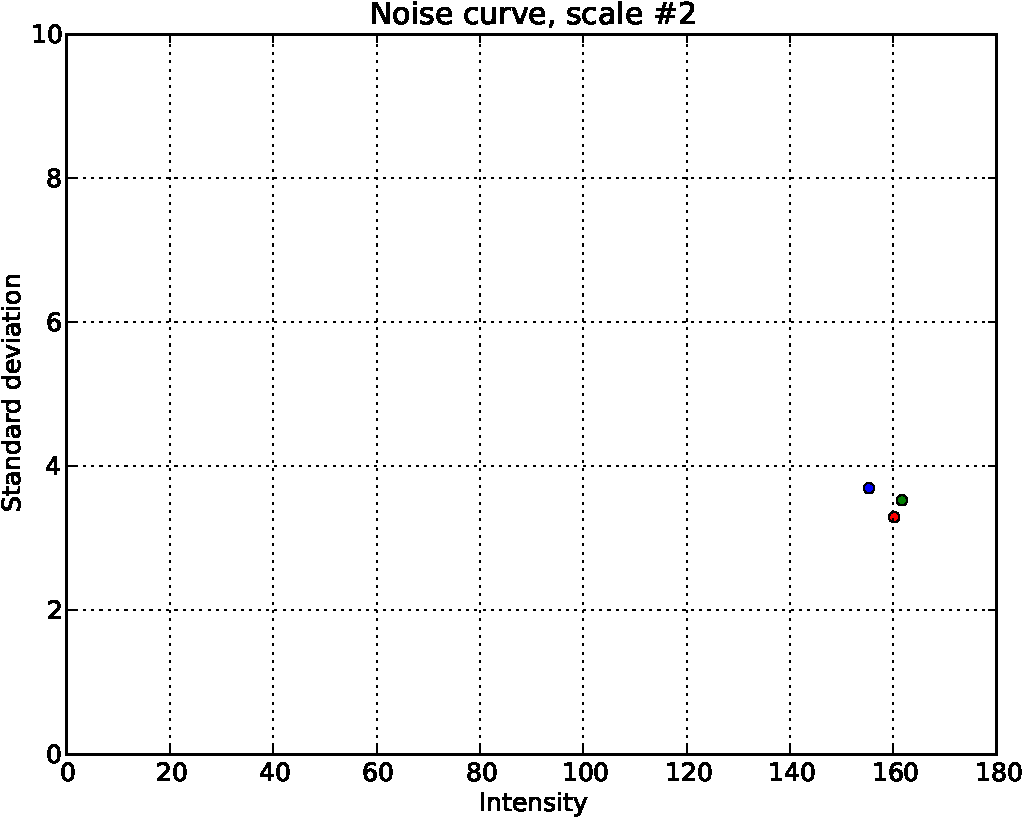
\includegraphics[width=.5\linewidth]{./images/curve.pdf}
\caption{This is an example of vector graphics. This figure is precise
  and well rendered at any zoom level on screens and printed with high
  resolution.}
\label{fig:example}
\end{center}
\end{figure}

You can produce vector PDF output with \verb|gnuplot| with proper options
(\verb|set terminal pdf|) and vector SVG figures the \emph{Inkscape}
program for example, and then convert them to PDF, or direct PDF output with
the PGF/TikZ \LaTeX\ packages\footnote{TikZ/PGF - Graphic systems for
  TeX, \url{http://pgf.sourceforge.net/}}. You can also convert EPS
vector images files to PDF files with the \verb|epstopdf| tool.
Simply converting a PNG file to PDF \emph{does not} create a vector
graphic file.

\subsection{Copyright}

Authors must warrant to be the authors of every part of the final
article including the images, or must include permission of the
copyright holder. If you use images you do not own, you must include
their authors and permissions to be used in the article in a special
section at the end of the article. We want other researchers to be
able to reuse these images for comparisons in other articles; try to
use only images under a permissive license like ``CC-BY'' or ``CC0''.

%------------------------------------------------------------------------------
\section{References}

We recommend the use of BibTeX with the SIAM bibliographic
style\footnote{The \verb|siam.bst| style file is available from
  \url{http://www.siam.org/journals/auth-info.php}.} for the automatic
formatting of the references. Reference presentation rules are
complex, see \emph{The Chicago Manual of Style} for
details\footnote{Extracts are available online at
  \url{http://www.chicagomanualofstyle.org/tools_citationguide.html}
  and \url{http://www.lib.sfu.ca/help/writing/chicago-turabian}.}.

References must include, at least: author(s), title,
journal/series/editor, volume, pages, year, and DOI/ISBN\@. Do
not use shortened journal titles.

Journal articles references must mention the DOI if it exists, presented
as ``\url{https://doi.org/AA.BBBB/CCCCCCC}'' at the end of the
reference block\footnote{See the Crossref DOI Display Guidelines at
  \url{http://www.crossref.org/02publishers/doi\_display\_guidelines.html}.}.
In BibTeX files, add the DOI in a \verb|note| field: \verb|note = {\url{https://doi.org/10.5201/ipol.2013.90}}|.

DOIs provides reliable and permanent links to the officially published
version of articles, and they are used by reference management tools
and indexing services to automatically collect reference citations
from a document. You can find DOIs for most of the published articles
using \href{http://www.crossref.org/guestquery/}{the Crossref Guest
  Query tool}.

Book references must mention the ISBN, presented as
``ISBN~XXXXXXXXXX'' at the end of the reference block. You can find
ISBNs for every published book in \href{http://isbndb.com/}{ISBNdb} or 
\href{http://www.worldcat.org/advancedsearch}{the WorldCat catalog}.

Grammatically, reference numbers may be treated like footnotes or
like nouns:
"\emph{Facchinei and Lucidi~[19] proved rate of convergence
  results; For recent convergence results, see~[19]; In~[19] results
  on the rate of convergence; as shown by Faccinei et Lucidi~[19]}".

Do not insert reference in the abstract. Instead, replace citations
with the reference itself, in brackets and formatted as follows:
\begin{description}
\item[Journal articles:]
  [P. T. Smith, K. Wang and J. W. Jones, SIAM Journal of Numerical
  Analysis, 26 (1989), pp. 600–623]
\item[Books:]
  [R. Doe and E. Prince, Principles of Physics, K. Lev, ed.,
  Birkhäuser, Basel, 1997]
\end{description}
If you refer by name to the authors of a cited work, you don’t need
to repeat the names within the reference: "\emph{In this paper we give
  an analysis of the algorithm by Smith, Prince, and Doe [SIAM Journal
    on Optimization, 9 (1999), pp. 755–778] for the solution of
  nonlinear large-scale problems.}"

Group references together: \verb|\cite{foo,bar}| instead of
\verb|\cite{foo}, \cite{bar}|.

Examples are included in bibliography, at the end of this document, for
journal articles~\cite{article}, preprints~\cite{preprint}, conference
papers~\cite{conference} and books~\cite{book}.

References to materials not formally published under editorial
control, such as websites, personal home pages, Wikipedia, etc.\ must
be provided in footnotes, not included in the References section. For example:

\begin{description}
\item[Wikipedia:]
  the photoelectric effect\footnote{Wikipedia,
    http://en.wikipedia.org/w/index.php?title=Photoelectric\_effect\&oldid=592445603 (3 February 2014)}
  is explained by \ldots
\item[Other web sites:]
  our implementation uses the GSL library\footnote{
GSL - GNU Scientific Library, \url{https://www.gnu.org/software/gsl/}
(10 March 2013)} to compute \ldots
\end{description}

%------------------------------------------------------------------------------
\section*{Acknowledgment}

Include an acknowledgment of grant and funding organizations at the
end of the article. For example: This work was partially funded by the
ONR grant 1234ABCD, ERC grand 5678XYZ, and Treilles Foundation.

%------------------------------------------------------------------------------
\section*{Image Credits}

You must mention the origin of \emph{every} image included in the article,
with their authors and license. Use a small font size for this
section, and set the heigh of the thumbnails to \verb|2em|. For example:\\
{\small

\includegraphics[height=2em]{images/finger.png}
  Glenn J. Mason (Flickr),
  CC-BY-SA\footnote{\url{http://www.flickr.com/photos/glennji/3558118429/}}\\     
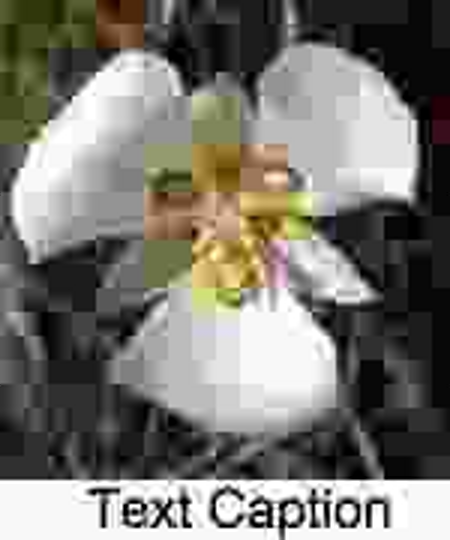
\includegraphics[height=2em]{images/lily.png}
  Lulu of the Lotus-Eaters (Wikipedia),
  CC-BY-SA\footnote{\url{http://en.wikipedia.org/wiki/File:Sego\_lily\_cm-150.jpg}}\\
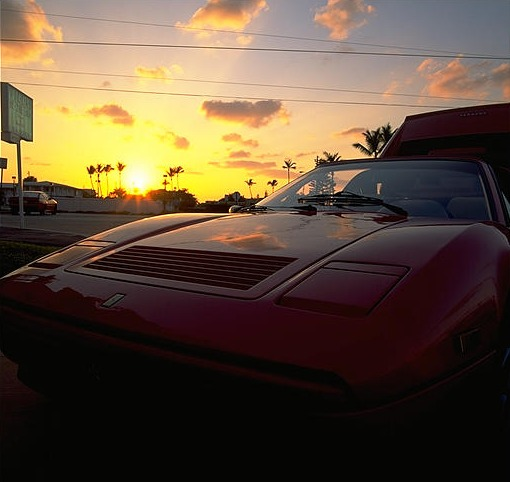
\includegraphics[height=2em]{images/ferrari.png}
  Courtesy Philip Greenspun\footnote{\url{http://philip.greenspun.com}}\\
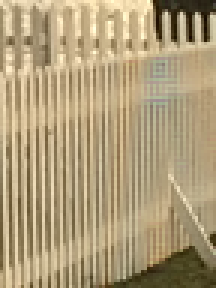
\includegraphics[height=2em]{images/k19.png}
  Kodak Image Suite\footnote{\url{http://r0k.us/graphics/kodak/}} \\
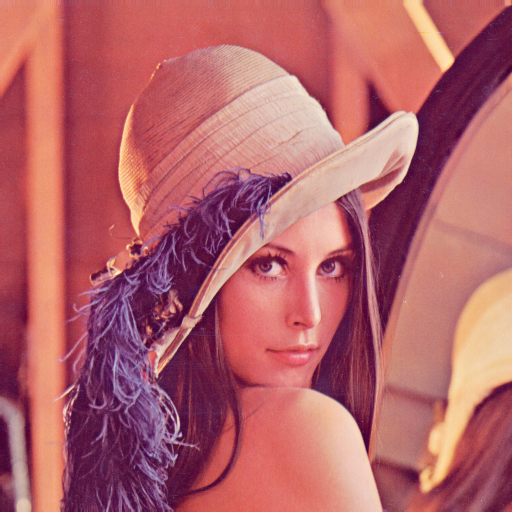
\includegraphics[height=2em]{images/lena.png}
  Standard test image
}

%------------------------------------------------------------------------------

\bibliographystyle{siam}
\bibliography{article}

\end{document}
%------------------------------------------------------------------------------
